
%\setcounter{chapter}{2}


\begin{Large}
\noindent
{\bf Lecture 2 \newline
Linear Vector Space 1}
\end{Large}
\vspace{1 cm}

\begin{list}{}{Chapter readings:}
\item Shankar ch 1
\item Sakurai 1.2, 1.3, 1.5
\item Cohen-Tanoudji ch 2A - 2E
\end{list}

 


\noindent
{\bf Definition:} A linear vector space $V$ is a collection of objects $\psi_{a}$, $\psi_{b}$, ...., called vectors, which satisfy the following postulates:
\begin{enumerate}
%\begin{list}{•}{•}
\item  If $\psi_{a}$ and $\psi_{b}$ are vectors in $V$, there is a unique vector $\psi_{a} + \psi_{b}$ in $V$, called the sum of $\psi_{a}$ and $\psi_{b}$. In other words, an operation called addition is defined in the vector space such that the space is closed under addition.

\item  The vector addition is commutative and associative, i.e.,
% add more space around the equal sign
$$\psi_{a} + \psi_{b} = \psi_{b} + \psi_{a}$$
$$\psi_{a} + (\psi_{b} + \psi_{c}) = (\psi_{a} + \psi_{b}) + \psi_{c}$$

\item  There is a vector in $V$ called the null vector and denoted by $\phi$ satisfying
$$\psi_{a} + \phi = \phi + \psi_{a} = \psi_a$$
for every $\psi_{a}$ in $V$.

\item  For every vector $\psi_{a}$ in $V$ there is another vector $\psi_{a}^{\prime}$ in $V$ such that
$$\psi_{a} + \psi_{a}^{\prime} = \phi$$
We denote $\psi_{a}^{\prime}$ as $-\psi_{a}$.

Note: We use the notation $\psi_{a} - \psi_{b}$ to mean $\psi_{a} + (-\psi_{b})$

\item  If $\psi_{a}$ is a vector and $\lambda$ is an arbitrary number (real or complex), called a scalar, there is a uniquely defined vector $\lambda\psi_{a}$ in $V$ satisfying:
\begin{description}
\item [(a)] $\lambda(\psi_{a} + \psi_{b}) = \lambda\psi_{a} + \lambda\psi_{b}\hspace{4mm}$ i.e., multiplication is distributive with respect to vector addition

\item [(b)] $(\lambda\mu)\psi_{a} = \lambda(\mu\psi_{a})\hspace{16mm}$ i.e., multiplication by a scalar is associative

\item [(c)] $(\lambda + \mu)\psi_{a} = \lambda\psi_{a} + \mu\psi_{a}\hspace{6mm}$ i.e., multiplication is distributive with respect to addition scalars

\item [(d)] Multiplication by scalars 0 and 1 are defined by
$$0\psi_{a} = \phi$$
$$1\psi_{a} = \psi_{a}$$
for any $\psi_{a}$ in $V$.
\end{description}
\end{enumerate}
% done so far




\section{Examples of linear vector space}

\begin{enumerate}
\item  Consider all real numbers $x$ in the range $-\infty$ to $\infty$, i.e.,
$$-\infty < x < \infty $$
$$x \in  \R$$
Take any two real numbers $x_{1}$ and $x_{2}$. If we add two real numbers we get another real number in $\R$. Thus,
$$x_{1} + x_{2} \in \R$$
Next take any real number $x$. If we multiply $x$ by another real number $\lambda$, we get a real number in $\R$, i.e.,
$$\lambda x \in \R$$
If we take a real number $x$, then there exists another real number $-x$ such that 
$$x + (-x) = 0$$
so the real numbers form a vector space with the real number themselves as vectors in the space. The number 0 is the null vector $\phi$ of the space. The scalars $\lambda$ by which the vectors are multiplied are also real numbers.

Thus the real numbers form a real linear vector space over a field which are also real numbers. The addition and multiplication are just the normal addition and multiplication of real numbers.


\item  The set of n-tuples of numbers ($x_{1}$, $x_{2}$, ...., $x_{n}$) when the addition of vectors and multiplication by a scalar are defined by
$$(x_{1},x_{2},.....,x_{n}) + (y_{1},y_{2},.....y_{n}) = (x_{1}+y_{1},x_{2}+y_{2},.....,x_{n}+y_{n})$$
and
$$\lambda(x_{1},x_{2},.....,x_{n}) = (\lambda x_{1},\lambda x_{2},.....,\lambda x_{n})$$


\item  The collection of all square-integrable complex valued functions of a real variable form a vector space. Consider all functions
$$ f: \R  \rightarrow \mathbb{C}$$
where $\R$ is the set of real numbers and $\mathbb{C}$ is the set of complex numbers, such that
$$\int_{-\infty}^{\infty} f^\ast(x)f(x)dx \equiv \int_{-\infty}^{\infty} \abs{f(x)}^2dx < \infty \hspace{5mm} \text{(i.e., finite).}$$
The sum of two functions and the product of a function by a complex scalar are defined in the usual way.

\hspace{5mm}The reason the square-integrable functions form a (complex) vector space is that the space is closed under addition. In other words, it can be shown that if $f$ and $g$ are two vectors, in this case two functions $f(x)$ and $g(x)$ both of which are square integrable, then $f(x) + g(x)$ is also square-integrable and hence the sum belongs to the vector space.

{\bf Proof:} Let $f(x)$ and $g(x)$ be two square-integrable functions, i.e.,

$$\int_{-\infty}^{\infty} \abs{f(x)}^2dx < \infty \hspace{5mm} \text{and} \hspace{5mm} 
\int_{-\infty}^{\infty} \abs{g(x)}^2dx < \infty$$.
Then using the inequality
$$\int_{-\infty}^{\infty} \abs{f + g}^2dx \leq \Bigg[\sqrt{\int_{-\infty}^{\infty} \abs{f}^2 dx} + \sqrt{\int_{-\infty}^{\infty} \abs{g}^2 dx}\hspace{1mm}\Bigg]^2$$
it is obvious that 
$$\int_{-\infty}^{\infty} \abs{f+g}^2dx < \infty \hspace{5mm} \text{(i.e., finite).}$$

\item  The set of all $n\, \text{ x }\, n$ matrices with complex elements form a complex linear vector space. For illustration, let 
the vector space be the set of all $2\times 2$ complex matrices. Any $2\times 2$ matrix
$$A=\begin{pmatrix}
\mqty{a\\c} & \mqty{b\\d}
\end{pmatrix}$$
where the elements, $a$, $b$, $c$ and $d$ can in general be complex, belongs to the vector (complex) space. We have

$$\phi =
\begin{pmatrix}
\mqty{0\\0} & \mqty{0\\0}
\end{pmatrix}
$$

$$\mathbb{I} =
\begin{pmatrix}
\mqty{1\\0} & \mqty{0\\1}
\end{pmatrix}
$$




$$-A =
\begin{pmatrix}
\mqty{-a\\-c} & \mqty{-b\\-d}
\end{pmatrix},\hspace{5mm}
\lambda A =
\begin{pmatrix}
\mqty{\lambda a\\ \lambda c} & \mqty{\lambda b\\\lambda d}
\end{pmatrix}
$$

\end{enumerate}
% done so far






\section{Inner-product space or a unitary vector space}
\label{sec:innerproduct}

For a general linear vector space, product of vectors (i.e., multiplication of two vectors) need not be defined. However, we will restrict ourselves to spaces in which a scalar product or an inner product is defined. \par

A linear vector space is called unitary if a scalar product is defined in it. To every pair of vectors $\psi_a$ and $\psi_b$ in $V$ there corresponds a unique scalar (in general complex), called the scalar product. The scalar product is defined to have the following properties:

\begin{description}
\item {\bf (a)} $(\psi_a,\psi_b) = (\psi_b,\psi_a)^\ast$
\item {\bf (b)} $(\psi_a,\lambda\psi_b) = \lambda(\psi_a,\psi_b)$
\item {\bf (c)} $(\lambda\psi_a,\psi_b) = \lambda^\ast(\psi_a,\psi_b)$
\item {\bf (d)} $(\psi_a,\psi_b+\psi_c) = (\psi_a,\psi_b)+(\psi_a,\psi_c)$
\item {\bf (e)} $(\psi_a,\psi_a) \geq 0; \text{ the equality holds only if }\psi_a\text{ is the null vector}$
\end{description}

It follows from the above postulated properties of the scalar product, that the product is linear with respect to 
the second vector, i.e., the vector after the comma,, i.e.,

$$(\psi_a,\lambda\psi_b+\mu\psi_c) = \lambda(\psi_a,\psi_b)+\mu(\psi_a,\psi_c)$$

and anti-linear with respect to the first vector, i.e.,


$$(\lambda\psi_a+\mu\psi_b,\psi_c) = \lambda^\ast(\psi_a,\psi_c)+\mu^\ast(\psi_b,\psi_c)$$



\section{Examples of scalar product}

\begin{description}
\item {\bf Ex 1} Consider the vector space consisting of all square-integrable complex-valued functions of a real variable in the domain $[a,b]$. This space is denoted by $L^2[a,b]$.

Suppose $\quad \quad \quad \quad \quad \quad  f \in L^2[a,b]$

i.e., 
  $$\quad \quad \int_a^bf^\ast(x)f(x)dx \equiv \int_a^b\abs{f(x)}^2dx < \infty$$

We can define the scalar product of two vectors f and g as

$$(f,g) \stackrel{def}{\equiv} \int_a^bf^\ast(x)g(x)dx = \text{ complex number}$$

We can show

$$\abs{(f,g)} \leq \Bigg[\sqrt{\int_{a}^{b} \abs{f(x)}^2 dx}\hspace{1mm}\Bigg]\Bigg[\sqrt{\int_{a}^{b} \abs{g(x)}^2 dx}\hspace{1mm}\Bigg].$$

Since both $f$ and $g$ are square-integrable, $\abs{(f,g)}$ is finite, i.e., the scalar product of $f$ and $g$ exists. The scalar product defined above satisfies all the properties that a scalar product is postulated to have.

\item {\bf Ex 2.} Now consider the vector space consisting of n-tuples of complex numbers. Such a vector space is denoted as $\mathbb{C}^n$.

\hspace{5mm}A vector  $\psi_a \in \mathbb{C}^n$ may be expressed as

$$\psi_a = \begin{pmatrix} a_1 \\ a_2 \\ \vdots \\ a_n \end{pmatrix}.$$

The scalar product may then be defined as

\begin{align*}
(\psi_a,\psi_b) & \stackrel{def}{\equiv}
\begin{pmatrix}
    a_1^\ast & a_2^\ast & \hdots & a_n^\ast
\end{pmatrix}
\begin{pmatrix}
        b_1 \\  b_2 \\ \vdots \\ b_n 
\end{pmatrix}  \\
               & = \sum_{i=1}^{n} a_i^\ast b_i
\end{align*}

This scalar product also satisfies all the properties of a scalar product.



\item {\bf Ex 3.} Euclidean 3-space $\R^3$. The vectors of $\R^3$ are 3-tuples of real numbers which could be represented as column vectors. Thus if $\psi_a$ and $\psi_b$ are in $\R^3$,

$$\psi_a = 
\begin{pmatrix}
    a_1 \\
    a_2 \\
    a_3
\end{pmatrix} \quad a_i = \text{ real}
$$

$$\psi_b = 
\begin{pmatrix}
    b_1 \\
    b_2 \\
    b_3
\end{pmatrix} \quad b_i = \text{ real}
$$

We could define the scalar product of $\psi_a$ and $\psi_b$ as

\begin{align*}
(\psi_a,\psi_b) & \stackrel{def}{\equiv}
\begin{pmatrix}
    a_1 & a_2 & a_3
\end{pmatrix}
\begin{pmatrix}
    b_1 \\
    b_2 \\
    b_3
\end{pmatrix}  \\
               & = \sum_{i=1}^{3} a_i b_i
\end{align*}

This scalar product also has all the postulated properties of a scalar product.
\end{description}






% done so far
In case of the vector space $\R^3$, the vectors $\psi_a$ and $\psi_b$ could be represented as directed lines $\vec{a}$ and $\vec{b}$ in a three-dimensional coordinate system as shown in the figure below:
\begin{figure}[ht]
\centering
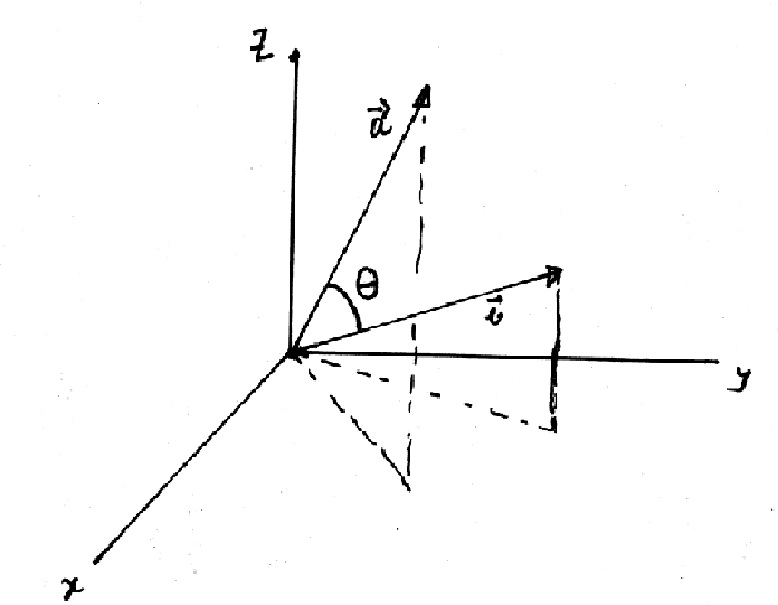
\includegraphics[width=100 mm]{euclid3vector.jpg}
\caption{A vector in the Euclidean three-space is represented by a directed line}
\end{figure}

\begin{flushleft}
The scalar product $(\psi_a,\psi_b)$ is the usual dot product
\end{flushleft}

\begin{align*}
\vec{a}.\vec{b} &= a_1 b_1 + a_2 b_2 + a_3 b_3 \\
               &= |\vec{a}| |\vec{b}| cos \theta
\end{align*}
where $|\vec{a}|$ and $|\vec{b}|$ are the magnitudes of the vectors $\vec{a}$ and $\vec{b}$ defined as

$$|\vec{a}| \equiv \sqrt{(\psi_a,\psi_a)} = \sqrt{a_1^2 + a_2^2 + a_3^2}$$
$$|\vec{b}| \equiv \sqrt{(\psi_b,\psi_b)} = \sqrt{b_1^2 + b_2^2 + b_3^2}$$


\section{Norm of a vector}

If a vector space is endowed with a scalar product, then the scalar product gives us the concept of the `magnitude' or `length' of a vector. In a general vector space the `magnitude' or `length' of a vector is called the norm of the vector. We simply define the norm of a vector $\psi_a$ as

$$\norm{\psi_a} \stackrel{def}{\equiv} \sqrt{(\psi_a,\psi_a)} $$

\begin{flushleft}
The norm has the following properties:
\end{flushleft}

\begin{description}
\item {\bf (a)} $\norm{\psi_a} \geq 0$, the equality holds only if the vector is null
\item {\bf (b)} $\norm{\psi_a + \psi_b} \leq \norm{\psi_a} + \norm{\psi_b}$, this is called the triangle inequality
\item {\bf (a)} $\norm{\psi_a - \psi_b} = \norm{\psi_b - \psi_a}$
\end{description}


\section{Metric induced by the scalar product}

The norm induced by the scalar product allows us to develop the concept of `distance' between vectors in a vector space. We say two vectors $\psi_a$ and $\psi_b$ are `close' if

$$\norm{\psi_a - \psi_b}$$
is small. The metric in a vector space assigns a real number to the vector $\psi_a - \psi_b$. This real number is a measure of how close the two vectors are. We simply define the metric $d(\psi_a,\psi_b)$ as

$$d(\psi_a, \psi_b) \stackrel{def}{\equiv} \norm{\psi_a - \psi_b}$$
Thus, if there are three vectors $\psi_a$, $\psi_b$ and $\psi_c$ and if $d(\psi_a,\psi_b) < d(\psi_a,\psi_c)$, then we say $\psi_a$ is closer to $\psi_b$ than to $\psi_c$.

\section{Schwarz inequality}

We will now prove a very important inequality called Schwarz inequality which states

\begin{flalign*}
&& \abs{(\psi_a, \psi_b)} &\leq \sqrt{(\psi_a, \psi_a)(\psi_b, \psi_b)}&\\
\text{or} && \abs{(\psi_a, \psi_b)} &\leq \norm{\psi_a} \norm{\psi_b}&\\
\end{flalign*}
{\bf Proof}

\begin{flalign*}
\text{Let}  && \psi        &= \psi_a + \lambda\psi_b &\\
\text{Then} && (\psi,\psi) &= (\psi_a + \lambda\psi_b, \psi_a+\lambda\psi_b)&\\
            &&             &= (\psi_a,\psi_a) + \lambda(\psi_a,\psi_b) + \lambda^\ast(\psi_b,\psi_a) + \abs{\lambda}^2(\psi_b,\psi_b) \geq 0
\end{flalign*}
The best inequality is obtained if $\lambda$ is chosen so as to minimize the left hand side of the above equation. By differentiation, the value of $\lambda$ which accomplishes this is found to be

$$\lambda = - \frac{(\psi_b,\psi_a)}{(\psi_b,\psi_b)}$$
Substitute this value of $\lambda$ in the above equation yields the Schwarz inequality. We note that the equality sign holds if and only if $(\psi,\psi) = 0$, i.e., $\psi$ is the null vector, i.e., $\psi = \phi$, in other words

\begin{flalign*}
&&\psi_a + \lambda\psi_b  &= \phi \text{ (null)}&\\
\text{i.e.} && \psi_a &= -\lambda\psi_b + \phi &\\
\text{or}   && \psi_a &= -\lambda\psi_b
\end{flalign*}
Hence, the equality holds if $\psi_a$ and $\psi_b$ are multiples of each other, or if $\psi_a$ and $\psi_b$ are ``parallel". It follows from the Schwarz inequality that the scalar product $(\psi_a,\psi_b)$ is finite if the norms of $\psi_a$ and $\psi_b$ are finite.

\section{Analogy of Schwarz inequality with vectors in a three-dimensional Euclidean space $\R^3$}

In $\R^3$, the vectors can be represented by directed lines (i.e., arrows). We have the scalar product of ordinary vectors in the form

$$\vec{A}.\vec{B} = \abs{\vec{A}}\abs{\vec{B}} \cos \theta.$$
Since cosine of any angle lies between -1 and 1, we have

$$\abs{\vec{A}.\vec{B}} \leq \abs{\vec{A}}\abs{\vec{B}}$$
The analogue of this equation for a general vector space is the Schwarz inequality:

$$\abs{(\psi_a, \psi_b)} \leq \norm{\psi_a} \norm{\psi_b}$$

% Done so far



\section{Orthogonality and linear independence}

A vector whose norm is unity is called a unit vector. For any given non-null vector, a unit vector can be formed by dividing the vector by its norm. Thus

$$u_a = \frac{\psi_a}{\norm{\psi_a}}$$
is normalized.

Two vectors $\psi_a$ and $\psi_b$ are orthogonal if their inner product is zero, i.e., if

$$(\psi_a,\psi_b) = 0.$$
The unit vectors $u_1$, $u_2$, ..., $u_N$ form an orthonormal set if they are mutually orthogonal, i.e., if

$$(u_i,u_j) = \delta_{ij}, \quad i,j = 1,2, \cdots , N.$$

\subsection{Linear Independence}

The set of vectors $\psi_1, \psi_2, \ldots , \psi_N$ are linearly independent if none of them can be expressed as a linear combination of the others. Mathematically this means that the equation

$$\sum_{j=1}^{N} c_j \psi_j = 0$$
cannot be satisfied except by $c_j = 0$ for all $j$.

\subsection{Orthonormality and linear independence}

A set of mutually orthogonal vectors (not necessarily normalized) are necessarily linearly independent. The converse is not true, however. That is, a set of linearly independent vectors may not be mutually orthogonal.

It is always possible to orthonormalize a set of linearly independent vectors. By this we mean that from a given set of $N$ linearly independent vectors, it is possible to form a set of $N$ orthonormal vectors. This procedure is called Schmidt orthonormalization method.



\subsection{Schmidt orthonormalization method}

Suppose $\psi_1, \psi_2, ..., \psi_N$ is a set of linearly independent vectors. Let
\be
u_1= \frac{\psi_1}{\norm{\psi_1}}.
\ee
Note that $u_1$ is normalized, i.e., $(u_1,u_1)=1$. Next construct the vector $\psi_{2}^{\prime}$ as follows:

\be
\psi_{2}^{\prime} = \psi_2 - u_1(u_1,\psi_2) ,
\ee
i.e., to obtain $\psi_{2}^{\prime}$ we have subtracted the `component' of $\psi_2$ along the $u_1$ ``direction''. Then it follows that
\begin{eqnarray*}
(u_1,\psi_2^{\prime}) &= &(u_1,\psi_2) - (u_1,u_1)(u_1,\psi_2) \\
                      &=& (u_1,\psi_2) - (u_1,\psi_2)       \\
                      &=& 0,
\end{eqnarray*}
i.e., $\psi_2^{\prime}$ is orthogonal to $u_1$. We then normalize $\psi_2^{\prime}$, i.e.,
\be
u_2 = \frac{\psi_2^{\prime}}{\norm{\psi_2^{\prime}}}.
\ee

\paragraph{}
We can continue the process until we exhaust all the vectors. For example, in the next step we can write
\be
\psi_3^{\prime} = \psi_3 - u_1(u_1,\psi_3) - u_2(u_2,\psi_3).
\ee
We note immediately that $\psi_3^{\prime}$ is orthogonal to both $u_1$ and $u_2$, i.e.,
$$(u_1, \psi_3^{\prime}) = (u_2,\psi_3^{\prime}) = 0$$
We normalize $\psi_3^{\prime}$ to get $u_3$, i.e.,
\be
u_3 = \frac{\psi_3^{\prime}}{\norm{\psi_3^{\prime}}}
\ee
Finally, in the $N^{th}$ step, we write
$$\psi_N^{\prime} = \psi_N - u_1(u_1,\psi_N) - u_2(u_2,\psi_N) - .... - u_{N-1}(u_{N-1},\psi_N)$$
$\psi_N^{\prime}$ is orthogonal to $u_1, u_2, ..., u_{N-1}$, i.e.,
$$(u_1,\psi_N^{\prime}) = (u_2,\psi_N^{\prime}) = ..... = (u_{N-1},\psi_N^{\prime}) = 0$$
Normalizing $\psi_N^{\prime}$ we get
\be
 u_N = \frac{\psi_N^{\prime}}{\norm{\psi_N^{\prime}}}.
\ee
Thus, the set $\{u_1,u_2,...,u_N\}$ is an orthonormal set of vectors.


% Done so far

\subsection{Dimension of a vector space}

The vector space $V$ is said to be $n$-dimensional if there exists $n$ linearly independent vectors, but if $n+1$ vectors are linearly dependent. The dimension may be finite or infinite.




\section{Complete vector space}

Before defining what a complete vector space is, we will give some other necessary definitions.

A sequence of vectors ${\psi_n}$ in the vector space $V$ is called a Cauchy sequence if for every $\epsilon > 0$ there exists 
an integer $N$ such that

$$\norm{\psi_n-\psi_m} < \epsilon$$
if $n,m>N$. In other words, the vectors in the sequence come `closer' if the index increases.

\begin{flushleft}
In particular
\end{flushleft}
$$\norm{\psi_n-\psi_m} \rightarrow 0 \text{ as } n,m \rightarrow \infty$$



\subsection{Convergence of a sequence of vectors in a vector space}

A sequence ${\psi_n},  n=1,2,...$ in a vector space $V$ converges to a vector $\psi$ in $V$ if for every $\epsilon > 0$ there exists an integer $N$ such that

$$\norm{\psi - \psi_n} < \epsilon$$
if $n>N$. That is, if

\begin{flalign*}
&& \lim_{n\rightarrow\infty}\norm{\psi - \psi_n} &= 0  &\\
\text{or} && {\psi_n} \rightarrow \psi,
\end{flalign*}
and the sequence is called a convergent sequence.

\noindent 
Now, we can show every convergent sequence is a Cauchy sequence.


\flushleft{\textbf{Proof}}
\begin{flalign*}
\text{Let}  && {\psi_n} &\rightarrow \psi &\\
\text{Then} && \norm{\psi_n-\psi_m} &= \norm{\psi_n-\psi+\psi-\psi_m}&\\
            &&                      &\leq \norm{\psi_n-\psi} + \norm{\psi-\psi_m} & \text{(triangle inequality)}
\end{flalign*}
Since $\{\psi_i, i=1,2, \cdots\}$ is a convergent sequence, each term on the right hand side tends to zero as $n$ and $m$ tends to infinity. 
Hence $\norm{\psi_n-\psi_m}\rightarrow 0$ as $n, m \rightarrow \infty$, i.e., the sequence $\{\psi_i, i=1,2,\cdots\}$ is a Cauchy sequence.


\paragraph{}
The converse of the above statement is not true in general. In other words, a Cauchy sequence in a vector space may not converge to a vector in the space. It can be shown that for a finite dimensional vector space the converse is true, i.e., in a finite 
dimensional vector space a Cauchy sequence is always a convergent sequence. Exceptions may arise in infinite dimensional vector space.




\subsection{An example of a vector space where Cauchy sequence does not converge to a vector in the vector space}

Consider the vector space consisting of all continuous functions of a single real variable $x$ in the range $[-1,1]$. In this vector space consider the
sequence $\{f_k(x), k = 1,2,\cdots\}$ of the following form:

\[
 f_k(x) = 
  \begin{cases} 
   1                    & \text{for } \frac{1}{k} \leq x \leq 1      \\
   \frac{kx+1}{2}       & \text{for } -\frac{1}{k} < x < \frac{1}{k} \\
   0                    & \text{for } -1 \leq x \leq -\frac{1}{k}
  \end{cases}
\]

$$k=1,2,3....$$

The graph of the sequence of functions is shown in Fig. (\ref{fig:sequence}) below.
\begin{figure}[ht!]
\centering
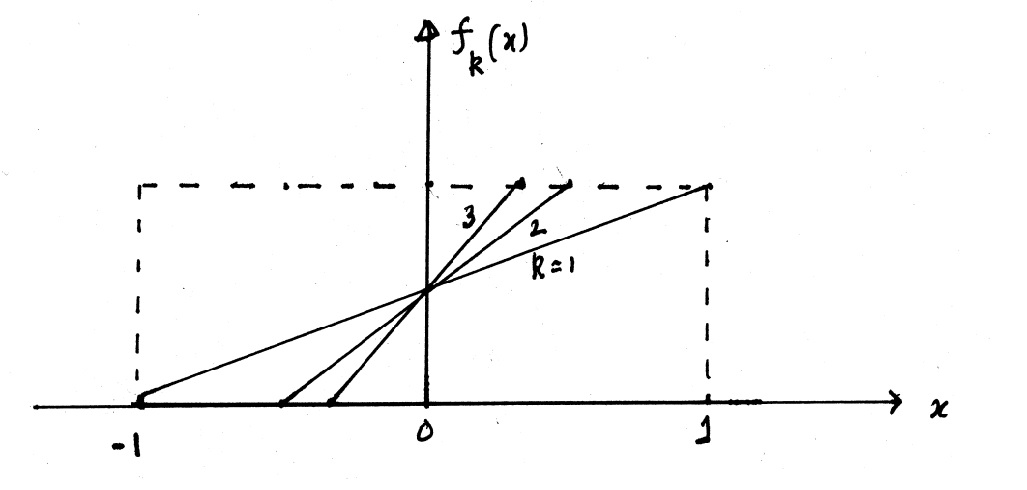
\includegraphics[width=\linewidth]{fig2.jpg}
\caption{A sequence of continuous functions converging to a discontinuous function}
\label{fig:sequence}
\end{figure}


Note that, in this example each $f_k(x)$ is continuous, but their first derivatives are discontinuous.

Let us define the scalar product in this space as

$$(f,g) = \int_{-1}^{+1} f^{\ast}(x) g(x) dx $$
so that the metric $d(f,g)$, i.e, the ``distance"   between the vectors $f$ and $g$ can be defined as
\[
d(f,g) \equiv || f-g || = \sqrt{ \int_{-1}^{+1} \left( f^*(x)-g^*(x)\right)\left( f(x)-g(x)\right) dx }. \]
With this metric we can show that the sequence $\{f_k\}$ defined above is indeed a Cauchy sequence. However, looking at the graph above, we see that as $k$ becomes large, $f_k$ approaches the $\theta$ function

\[
 \theta(x) = 
  \begin{cases} 
   0    & \text{for } x < 0 \\
   1    & \text{for } x > 0 \\
  \end{cases}
\]
which is a discontinuous function at $x=0$. We show the graph of $\theta(x)$ below
\begin{figure}[ht!]
\centering
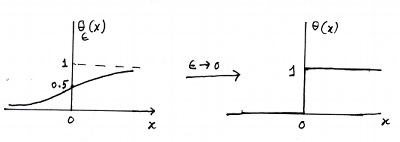
\includegraphics[width=80 mm]{theta.jpg}
\caption{The theta function.}
\end{figure}


Thus the Cauchy sequence $\{f_k(x)\}$ of continuous functions is converging to a discontinuous function which lies outside the vector space $V$ because the vector space was defined as the collection of all continuous functions.

\paragraph{}
If, instead of choosing all continuous functions, we had chosen all square integrable functions as defining the vector space, then any Cauchy sequence in the vector space would converge to a vector within the space.

\vspace{3 mm}
\textbf{Def: } A linear vector space is said to be \underline{complete} if any Cauchy sequence converges to a vector in the space.




\subsection{Hilbert Space}

A complete linear vector space, finite or infinite dimensional, endowed with a scalar product between vectors (and hence endowed with a norm and metric induced by the scalar product), is called a Hilbert space.

A finite-dimensional vector space is always complete. So, a finite-dimensional linear vector space in which a scalar product is defined is a Hilbert space.

An infinite dimensional vector space with a scalar product may or may not be complete. Whether or not an infinite-dimensional vector space is complete depends upon how exactly the vector space is defined and on the metric.

\section{Basis in a Hilbert space}

\subsection{Finite dimensional space}

In a finite dimensional vector space of dimension $n$, any set of  $n$ linearly independent vectors $\psi_1, \psi_2, ...., \psi_n$ spans the entire space. In other words, an arbitrary vector $\psi$ in the space can be expressed as a linear combination of $\psi_1, \psi_2, ...., \psi_n$, i.e.,

\be
\psi = \sum_{i=1}^{n} a_i \psi_i.
\ee
The vectors $\{ \psi_1, \psi_2, ...., \psi_n\}$ form a complete basis for the vector space. These vectors, even if linearly independent, may not be orthogonal to each other. It is more convenient to use a set of $n$ orthonormal vectors $\{ \phi_1, \phi_2, ...., \phi_n\}$ as the basis. Being orthogonal, the vectors 
$\{ \phi_1, \phi_2, ...., \phi_n \}$ are automatically linearly independent. The orthonormal set of basis vectors 
$\{\phi_i, i=1,2,...n\}$, can be constructed from the set $\{\psi_i,i=1,2, ...,n\}$ by using the Schmidt orthonormalization procedure.

\vspace{3mm}
\hspace{5mm}Choosing the orthonormal set as the basis, any vector $\psi$ in the vector space can be written as
\be
\psi = \sum_{i=1}^{n} a_i \phi_i 
\ee
where
\be
(\phi_i,\phi_j) = \delta_{ij}.
\label{eq:phi}
\ee
Using Eq. (\ref{eq:phi}), we have 
\be
a_i = (\phi_i,\psi).
\ee

%done so far

\subsection{Infinite-dimensional vector space}

In an infinite-dimensional vector space the number of basis vectors is infinity. Let $\{\phi_1,\phi_2,\phi_3,...\}$ be an infinite set of orthonormal basis vectors spanning the infinite-dimensional Hilbert space. This set of basis vectors is said to be \underline{complete} if \underline{any} vector $\psi$ in the Hilbert space can be expanded as a linear combination of the basis vectors, i.e.,

\be
\psi = \sum_{i=1}^{\infty} a_i \phi_i.
\label{eq:infsum}
\ee
In an infinite-dimensional vector space, choosing an infinite number of basis vectors may not ensure that the basis set is complete. It may so happen that there are other linearly independent vectors, may be infinite in number, which have been missed in the first choice of the basis vectors. Whenever we have an infinite sum, as in Eq. (\ref{eq:infsum}), the issue of convergence arises. We can understand
Eq. (\ref{eq:infsum}) in the sense that the sequences consisting of the partial sums
$$f_n = \sum_{i=1}^{n}a_i\phi_i \hspace{3mm} ; \hspace{3mm} n = 1, 2, 3,...$$
converges to $\psi$, i.e.,
\be
\lim_{n \rightarrow \infty} \norm{\psi - f_n} \rightarrow 0 
\ee
% Done so far
% need correction here
% what is limit of n?
Since the vector $\psi$ must have a finite norm, we must have
\be
\norm{\psi}^2 = (\psi,\psi) = \sum_{i=1}^{\infty} \abs{a_i}^2 < \infty \text{ (finite)} .
\label{eq:finite}
\ee
If the basis vectors $\phi_i$ are orthonormal, we have
$$a_i = (\phi_i, \psi),$$
so that Eq. (\ref{eq:finite}) can be written as
\be
\sum_{i=1}^{\infty}\abs{(\phi_i,\psi)}^2  < \infty .
\ee
The scalars $a_i$ can be regarded as the components of $\psi$ in the `directions' $\phi_i$.
\vspace{3mm}

%done so far

\underline{\textbf{Ex}}.  Show that the set of all square integrable functions, i.e., set of all functions $f$ such that 

$$\int_{-\infty}^{\infty} f^{\ast}(x)f(x)dx < \infty \text{  (i.e., finite)}$$
belong to a Hilbert space. This Hilbert space is denoted as $L^2(-\infty,\infty)$.

\vspace{3mm}

To show this, consider the following:

\begin{enumerate}
\item  If $f$ and $g$ are square integrable functions, so if $f+g$, and hence $f+g$ also belongs to the Hilbert space.
$$\norm{f+g} \leq \norm{f} + \norm{g}$$

\item  We can define the scalar product between $f$ and $g$ as follows:
$$(f,g) \stackrel{def}{\equiv} \int_{-\infty}^{\infty}f^{\ast}(x)g(x)dx$$
That the scalar product exists follows from the Schwarz inequality
$$\abs{(f,g)} \leq \norm{f}.\norm{g} < \infty$$

\item  It can also be shown that any Cauchy sequence of square integrable functions converges to a limit which is also square integrable. In other words, the space of all square integrable functions is complete.
\end{enumerate}

Hence the linear vector space consisting of all square integrable functions is indeed a Hilbert space.


% done so far

\section{Dirac Notation}
Cohen-Tannoudji, page 109. \newline
``Ket'' vectors a ``bra'' vectors. 
\vspace{3mm}

\textbf{\underline{Notation}}

\hspace{5mm}Any element, or vector of a vector space $V$ is called a \underline{ket vector}, or, more simply, a \underline{ket}. It is represented by the symbol $\ket{\hspace{1mm}}$, inside which is placed a distinctive sign which enables us to distinguish between different kets, for example $\ket{\psi}$.

\vspace{3mm}

\textbf{\underline{Scalar product}}

\vspace{1mm}

\hspace{5mm}With each pair of kets $\ket{\phi}$ and $\ket{\psi}$, taken in this order, we associate a complex number, which is their scalar product $(\ket{\phi}, \ket{\psi})$ and which satisfies various properties discussed earlier in section 
\ref{sec:innerproduct}.

\newpage

\textbf{\underline{Dual vector space}}

\vspace{1mm}

Linear functional:\newline
First we define the a linear functional. A linear functional $\chi$ is a linear operation on the kets such that $\chi$ operating on a ket $\ket{\psi}$ gives a complex scalar:
$$\chi \ket{\psi} \rightarrow \text{scalar, where } \ket{\psi} \in V$$
and
$$\chi (\lambda_1 \ket{\psi_1} + \lambda_2 \ket{\psi_2}) = \lambda_1 \chi \ket{\psi_1} + \lambda_2 \chi \ket{\psi_2}\text{.}$$
The set of all linear functionals defined on the kets of a vector space $V$ themselves form a linear vector space called the dual space of $V$ and symbolized by $V^{\ast}$.

\vspace{3mm}

\textbf{\underline{Bra notation for the vectors of $V^{\ast}$}}

\vspace{1mm}

\hspace{5mm}Any element, or vector, of the space $V^{\ast}$ is called a ``bra vector'', or, more simply, a bra. It is symbolized by $\bra{\hspace{1mm}}$. For example, the bra $\bra{\chi}$ designates the linear functional $\chi$. We shall henceforth use the notation $\braket{\chi}{\psi}$ to denote the number obtained by causing the linear functional $\bra{\chi} \in V^\ast$ to act on the ket $\ket{\psi} \in V$. Thus
$$\chi(\ket{\psi}) = \braket{\chi}{\psi}\text{.}$$




\textbf{\underline{Correspondence between kets and bras}}

\vspace{1mm}

\hspace{5mm}The existence of the scalar product in $V$ will now enable us to show that we can associate with every ket 
$\ket{\phi} \in V$ an element of $V^\ast$, that is a bra, which will be denoted by $\bra{\phi}$.

\hspace{5mm}The ket $\ket{\phi}$ does indeed enable us to define a linear functional, the one which associates with each $\ket{\psi} \in V$ a complex number which is equal to the scalar product $(\ket{\phi},  \ket{\psi})$. Let  $\bra{\phi}$ be this linear functional. It is thus defined by the relation
$$\braket{\phi}{\psi} = (\ket{\phi}, \ket{\psi})\text{.}$$


\newpage

\textbf{\underline{The correspondence is antilinear}}

\vspace{1mm}

Let $\lambda_1 \ket{\phi_1} +\lambda_2 \ket{\phi_2}$ be a ket. Then
\begin{flalign*}
&& (\lambda_1 \ket{\phi_1} +\lambda_2 \ket{\phi_2}, \ket{\psi}) &= \lambda_1^{\ast} (\ket{\phi_1},\ket{\psi}) + \lambda_2^{\ast} (\ket{\phi_1},\ket{\psi}) & \\
&& &= \lambda_1^{\ast} \braket{\phi_1}{\psi} + \lambda_2^{\ast} \braket{\phi_2}{\psi} & \\
&& &= (\lambda_1^{\ast}\bra{\phi_1} + \lambda_2^{\ast}{\bra{\phi_2}})\ket{\psi}
\end{flalign*}
Thus
$$\lambda_1 \ket{\phi_1} +\lambda_2 \ket{\phi_2}  \stackrel{dc}{\rightarrow} \lambda_1^{\ast}\bra{\phi_1} + \lambda_2^{\ast}{\bra{\phi_2}}$$
where ``dc'' is short for dual correspondence.

\vspace{3mm}

\textbf{\underline{Comment}}

\vspace{1mm}
\hspace{5mm} If $\lambda$ is a complex number and $\ket{\psi}$ is a ket, then $\lambda\ket{\psi}$ is also a ket. We are sometimes led to write $\lambda\ket{\psi}$ as $\ket{\lambda\psi}$:
$$\ket{\lambda\psi} = \lambda\ket{\psi}$$
One must be careful to remember that $\bra{\lambda\psi}$ represents the bra associated with the ket $\ket{\lambda\psi}$. Since the correspondence between a bra and a ket is antilinear, we have
$$\bra{\lambda\psi} = \lambda^\ast \bra{\psi}$$

\vspace{3mm}

\textbf{\underline{Dirac notation for the scalar product}}

\vspace{1mm}
\hspace{5mm} We now have at our disposal two distinct notations for designating the scalar product of $\ket{\psi}$ by 
$\ket{\phi}$, namely, $(\ket{\phi},\ket{\psi})$ and $\braket{\phi}{\psi}$, $\bra{\phi}$ being the bra associated with the ket $\ket{\phi}$.

We shall mostly use the Dirac notation $\braket{\phi}{\psi}$. In the table below we summarize, in Dirac notation, the properties of the scalar product:

\begin{enumerate}
\item  $\braket{\phi}{\psi} = \braket{\psi}{\phi}^\ast$
\item  $\braket{\phi}{\lambda_1\psi_1 + \lambda_2\psi_2} = \lambda_1\braket{\phi}{\psi_1} + \lambda_2 \braket{\phi}{\psi_2}$
\item  $\braket{\lambda_1\phi_1 + \lambda_2\phi_2}{\psi} = \lambda_1^\ast \braket{\phi_1}{\psi} + \lambda_2^\ast \braket{\phi_2}{\psi} $
\item  $\braket{\psi}{\psi} $ is real, positive; zero if and only if $\ket{\psi} = \phi $ (null).
\end{enumerate}

%%  Hooray


